 \chapter{Collaborative Filtering\index{Collaborative Filtering}}


\textsf{ In this chapter we explain Collaborative Filtering in more detail,
along with giving details of the NETFLIX prize and the lead up to present work.
We explain about the data and the approach to the solution of the problem.}


\section{Recommender Systems\index{Recommender Systems}}
Internet technologies have greatly become a part of our lives, there are many
occasions when we need help in taking certain decisions. Recommendations in
general is ubiquitous when there is a need to make choices without sufficient
personal experience, we rely on feedback from users on certain products, we make
use of recommendation letters for jobs, reviews of movies and books
\cite{Resnick:1997:RS:245108.245121}. Consider for a movie streaming company
like NETFLIX, where people can watch movies from a huge collection, have been
collecting the ratings of the movies from the users. This data can be considered
as our \emph{training data}, it is explicitly obtained from the users. Using
this training data the company makes predicitions of movies the users are likely
to prefer watching more than others. This is only one of the different types of
recommender systems. 
\subsection{Recommender System Strategies}
The strategies for building recommender systems are based on the type of data
available and how the data is used. On a broad sense the two main approaches are
\emph{content-based filtering}, in which the items are characterized based on 
certain attributes, and recommendation are made based on filtering similar
items. In the second approach, \emph{collaborative filtering}, the ratings
previously given by users is used to build a model, which is then used to make
predictions. The term Collaborative Filtering was first termed by Tapestry
\cite{Goldberg:1992:UCF:138859.138867}, which was one of the first recommender
systems. Recommender
Systems produce possibly accurate prediction of relationship between elements of
different classes based on previous knowledge or the \emph{training data}. This
training data could be explicitly obtained in the form of ratings given by
users or it could be implicit knowledge(purchase
history, browsing history, search patterns,mouse movements etc), which can be
used when explicit knowledge is insufficient \cite{Hu:2008:CFI:1510528.1511352}.
But however in this thesis work we model our system based on explicit
knowledge. 

Modern recommender systems are based on the collaborative filtering, which again
is of two types, the \emph{nearest neighbor approach} and the \emph{latent
factor approach}. In the nearest neighbor methods, items or users are given
certain attributes which decides the proximity between them. Further this sense
of proximity is used predict an item for an user. The second approach is
the latent factor approach, which characterizes the users and the items together
in building the model. Matrix factorization is used to build these models, likes
of SVD is very useful. \emph{Rating matrix} proves to be important, as it
charectarizes both items and users as its vectors. 

\subsection{The Problem Formulation}
Our problem could be defined as a matrix completion problem, where the matrix is
formed by placing the users $u$ along the rows and the movies $m$ along the
rows. The entries in this matrix are filled through the \emph{training data},
which is collection of $n$ \emph{quadruples}, with the format
(\emph{user(k)},\emph{movie(k)},\emph{rating(k)},\emph{timestamp(k)}), where
$k=1,2...,n$. The $1 \leq user \leq u$ and $1 \leq movie \leq m$ are the
range of the users and the movies, where as the ratings, $1<rating<5$. The
\emph{Rating
matrix} is defined as $R\in\mathbb{R}^{u,m}$, \\
\begin{equation}
  R[i,j]=\begin{cases}
    rating(k), & \text{$i=user(k), j=movie(k)$}.\\
    ?, & \text{otherwise}.
  \end{cases}
\end{equation}

where \emph{'?'} are the cases where the \emph{user-movie} relation is unknown.
These are the values which needs to be predicted. Once the \emph{'?'} values are
computed, recommendations could be made depending on the required tolerance
level, \emph{user-movie} pairs with predicted ratings higer than the tolerant
value(threshold) can be selected for making recommendations. Hence this problem
can be viewed as a \emph{matrix completion} problem. In this thesis work, we
will compute the unknowns for a certain subset called the \emph{test set}. \\

Let us denote the completed matrix, or rather the reconstructed matrix	by 
l\emph{$\hat_{R}$}. We intend to obtain the
\emph{$\hat_{R}$}, by reproducing it through a simple product of two matrices
with reduced \emph{inner dimension}. Let $P\in\mathbb{R}^{u,f}$ and
$Q\in\mathbb{R}^{f,m}$ are the two matrices with reduced inner dimension
\emph{f}. 

\section{NETFLIX}
Entertainment has been one of the most significant integral part of human
society and has evloved along with modern technologies. In todays internet
driven society, IPTV(Internet Protocol Television) is gaining popularity in
delivering television and cinema content to viewers. IPTV mainly consists of
three groups, \\
\begin{enumerate}%for small alpha-characters within brackets.
\item Live Television - Live telecast or transmission to the viewers with only
the transmission delay, example live news show.
\item Time-shifted Television which is also called as catch-up TV, in which the
viewers can watch the content which is stored and available at any point of
time. 
\item Video on Demand - here the viewers are given a wide range of TV shows and
movies to choose. They can watch anything they wish, the content is streamed to
the viewers computer which the user can pause and watch later. NETFLIX provides
its content throught this method. \\
\textbf{Netflix, Inc} is a company based in USA, which provides internet
streaming media on-demand. This owes to a great extent to the success of
NETFLIX, since through on Demand
system NETFLIX is able to cater to individual tastes of users. NETFLIX can
collect statistics pertaining to individual users' choices and the most
important metric is the \emph{ratings}. NETFLIX aims to greatly improve the
customer satisfaction and retention by providing a greatly personalised
experience to the users. The importance of personalization is such, that NETFLIX
ignited the research attempts in the Mathematical and Computer Science soceity
to develop methods which could do predictions for movie likeability quotient.
Such attempts have certainly been fruitful to NETFLIX as is evident from the
fact that as of today 33 million members view over 1 billion hours of TV shows
and movies through NETFLIX per month.
\end{enumerate}

\subsection{NETFLIX Prize}
During October 2006, NETFLIX challenged the research community to beat the
performance in terms of accuracy of their own recommendation system
\emph{Cinematch} by 10\%. The NETFLIX prize challenge was provided with over 100
million ratings from around half a million users and 18 thousand movies. This
data was collected during the period october 1998 and December 2005. The
challenge would take place over a period of three years, and a progress prize of
50 thousand USD would be awarded each year to the team which would produce the
best improvements. Finally at the end of three years a Grand Prize of 1 Million
USD would be given to the team with the best results in terms of RMSE. Their
benchmark system \emph{Cinematch}, based on \emph{Pearson correlation} which is
straightforward statistical linear model produces an RMSE of 0.9525 on test
data. Hence to qualify to win the Grand Prize which accounts for 10\%
improvement over \emph{Cinematch}, which corresponds to RMSE of 0.8563 on
\emph{quiz set}. On an event of a tie the time of entry would be taken into
account, and this is exactly what happened on 26 July 2009, team BellKor's
Pragmatic Chaos won the challenge by margin of 20 minutes. Table 2.1 shows the
performance of top 12 teams, \cite{NETFLIX_Prize:Online}
\begin{table}
\centering 
\begin{tabular}{|c|c|c|c|} \hline %\hline
%-------------------------------------------------------------------
$Rank$ & $Team$ & 
$RMSE$ &  $Percent Improvement$  \\ 
\hline
%-------------------------------------------------------------------
$ 1$
& $BellKor's Pragmatic Chaos$
& $0.8567$
& $10.06$ \\ %\hline
%-------------------------------------------------------------------
$ 2$
& $The Ensemble$
& $0.8567$
& $10.06$ \\ %\hline
%-------------------------------------------------------------------
$ 3$
& $Grand Prize Team$
& $0.8582$
& $9.90$\\  %\hline
%-------------------------------------------------------------------
$ 4$
& $Opera Solutions and Vandelay United$
& $0.8588$
& $9.84$\\  %\hline
%-------------------------------------------------------------------
$ 5$
& $Vandelay Industries !$
& $0.8591$
& $9.81$ \\%\hline
%-------------------------------------------------------------------
$ 6$
& $PragmaticTheory$
& $0.8594$
& $9.77$ \\ %\hline
%-------------------------------------------------------------------
$ 7$
& $BellKor in BigChaos$
& $0.8601$
& $9.70$ \\ %\hline
%-------------------------------------------------------------------
$ 8$
& $Dace$
& $0.8612$
& $9.59$ \\ %\hline
%-------------------------------------------------------------------
$ 9$
& $Feeds2$
& $0.8622$
& $9.48$  \\%\hline
%-------------------------------------------------------------------
$ 10$
& $BigChaos$
& $0.8623$
& $9.47$ \\ %\hline
%-------------------------------------------------------------------
$ 11$
& $Opera Solutions$
& $0.8623$
& $9.47$ \\ %\hline
%-------------------------------------------------------------------
$ 12$ 
& $BellKor$        
& $0.8624$ 
& $9.46$  \\ \hline 
\end{tabular}
\caption{RMSE of Top 12 Teams}
\label{tab:TopTeams}
\end{table}
-
\subsection{The NETFLIX dataset}
NETFLIX had been collecting data since October 1998,
as of June 2007 the company had collected over 1.9 billion ratings from more
than 11.7 million subscribers over 85 thousand titles \refname{The NETFLIX
Prize}. The company then recieved over 2 million ratings per day. To provide
data for the competition the company did two seperate random sampling processes,
the first one to obtain th eentire Prize dataset and second for the qualifying
and probe set. The condition for selecting the users was that they should have
given minimum of 20 ratings. \\

 Basically the company has seggregated the data based on time, the latest data
form the Test Data and the initial data form the training data. The
\emph{Training data} includes the \emph{Probe set} which is meant for fine
tuning before submissions. The training data is basically a text file consisting
of triplets entries like, (UserID, MovieID, Rating). There are 100 million such
entries which form the training set. The training set also included the probe
set consisting of 1,408,395 triplets, this could be used by the competitors to
fine tune their algorithms before submission. NETFLIX also collected the latest
ratings of all the users in the training set to form the \emph{Qualifying set}.
This set was in the form (UserID,MovieID,DatrofRating), where the ratings were
known only to the judjes. The qualifying set was again divided into 2 groups,
the \emph{Quiz set} and \emph{Test set}. The quiz set having 1,408,342 ratings
was used to update the Leaderboard, the RMSE on this quiz set was released to
the competitors. The test set having 1,408,789 ratings was only used by the jury
to adjudge the winner. \cite{Bennett07thenetflix}\\



 
\begin{table}
\begin{center}
    \begin{tabular}{|ccc|}
        \hline
         TRAINING SET  & ~ &  Probe set  \\ 
         100480507 & ~ & 1408395   \\ \hline       
    \end{tabular} \\
    \caption[]{Training Data}
     \begin{tabular}{|c|c|}
       \hline
       Test Set  & Quiz Set  \\ 
       1408789 & 1408342 \\ \hline       
    \end{tabular}
    \caption{Qualifying Data}     
\end{center}
\end{table}

\section{Temporal Dynamics in NETFLIX data}
The main goal in this work is to integrate temporal information into the
Recommender System model we are building based on collaborative filtering. It is
very important to consider temporal dynamics since the vast amounts of data we
are flooded with is dynamic in nature, and most of the information retrieval
tools today consider only the snapshot of this data, thereby loosing one very
potential dimension. In this chapter we present in detail the significance of
temporal dynamics in general and with respect to NETFLIX and also how to include
temporal dynamics into the model. \\


Since we are trying to improve the prediction rate by including temporal
effects, it is very critical to identify and uncover all possible temporal
effects within the NETFLIX data. This section summarizes and reports the
temporal analysis of the NETFLIX data.

\section{Tracking Drifting Customer Preferences}
The phenomena of $Concept drift$ is evident in the case of NETFLIX system, as we
can see that the user preferences of movies keep changing over time due to
various reasons. Concept drift means when the statistical properties of the
target variables change with time, like how user preferences change with new
release of new movies. In our case where we are trying to collaborate using
interconnected preferences among users, it is a challenge since each of the
interacting users could be drifting in different ways and also they are in
different time instances. There are mainly three kinds of approaches to include
time apect, \emph{instance selection}, in which only the recent instances are
considered, discarding off other instances. All instances within a specific time
period is given equal opportunities discarding instances ouside this period.
This obviously leads to lose of information.  In 2005, a time-weighted CF method
was proposed by Ding and Li in \cite{Ding:2005:TWC:1099554.1099689}, in
which depending on how recent the ratings are they are weighted accordingly,
these models do include time but only as weighted schemes, this is the second
approach called \emph{instance weighting}. The third approach is the
\emph{ensemble learning}, in which predictions from number of models are
combined to give a final prediction. But in this approach, if each of the
individual predoctors capture local behaviour, the global patterns are
overlooked.  A more complex approach was proposed by Koren et al, in
\cite{Koren:2010:CFT:1721654.1721677}, in
which the various complex time parameters are incorporated into the model.
We have built our model based on the following guidelines, \\
\begin{itemize}
  \item We try to model for the entire time period, instead of any particular
instances or particular time periods.
  \item We try to capture the multiple drifts based on the user, both sudden
changes and gradual changes.
  \item All the various drifts will be combined into a single framework.
\end{itemize}

\begin{example}
 As an example consider two users Joe(21 years old) and John(41 years old)
rating a common movie Godfather(1972). During November 2008, Godfather was voted
No. 1 in Empire magazine's list of The 500 Greatest Movies of All Time. Joe
after seeing this watched the movie and gave his rating. On the other hand John
had rated the movie 20 years back. This makes them both roughly the same age
when they have rated the movie, however in a different time instance. It is
clear that Joes rating could have had certain bias caused by $classical$ nature
of the movie.
\end{example}

\section{Temporal Dynamics in NETFLIX Data}
Here we would show through plots the dynamic nature inherent in the data with
respect to time. 


\begin{figure}[h]
\centering
\subfigure[Movie Means by Date]{
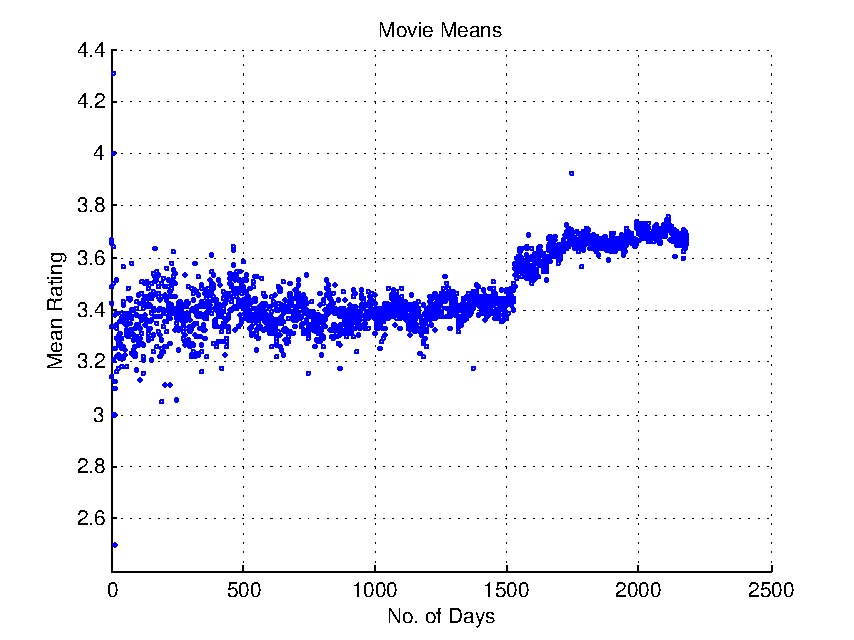
\includegraphics[width=0.45\textwidth]{./New/MovieMeans_AllMovie.pdf}
\label{fig:MovMean}
}
\subfigure[Movie Means by Movie Age]{
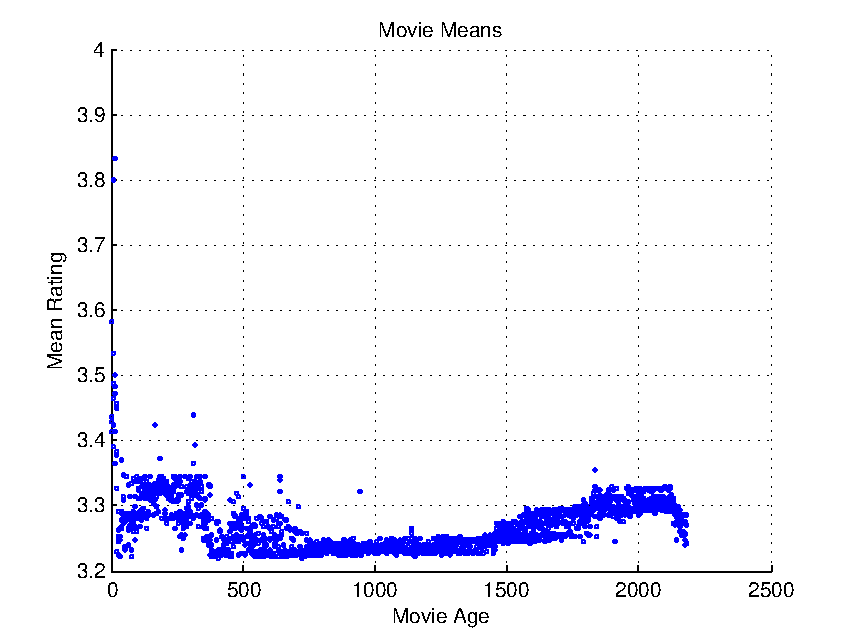
\includegraphics[width=0.45\textwidth]{./New/MovieMeans_AllMovie_Age.pdf}
\label{fig:MovMean_Age}
}\\

\label{fig:MovieMean_temporal}
\caption{Movie Means vs Time}
\end{figure}



\section{Temporal-Factor Model}
As we had seen in the previous chapter, that all the non user-item interaction
effects are encapsulated in the \emph{Baseline predictors}, we will show here
who we intend to include temporal baseline predictors. Here we explain the
theoretical analyses and findings related to various time changing aspects of
users and of movies. It is clear that the time dynamics of movies will be more
gradual than that of the users. The movies are analysed based on a large number
of users who have rated the single movie, but however as an individual user the
temporal analyses is done on large number of unrelated factors, hence the user
behaviour seems more complex and less uniform compared to the movies. \\
The main challenge is to parameterize the user-drift and the movie-drift as
appropriately as possible. The first and foremost consideration is how
transitory are the user-drift and the movie-drift. As we will expalin in detail
the movie-drift seems to be more uniform and less transient than the user-drift,
hence it is wise to consider finer time resolution to model user-drift and
coarser resolution for movies. The final model should however account for both
temporal effects spanning on a longer duration and the more transitory changes. 
For example, movies dont change on a daily basis, some of the factors which
could affect the movies dont occur often like appearance of an actor in another
movie, or the movie winning an award or the movie recieving appreciation from a
critique. On the contrary consider an user, who usually rates relative to other
ratings, so his rating scale could vary everytime he has seen on influencing
movie proir to the current movie of interest. A user who usually rate 4 for
average movies, could be influenced to rate the same kind of average movies by
3. \\

\begin{figure}[h!]
\centering
\subfigure[Monthly Average of All movies]{
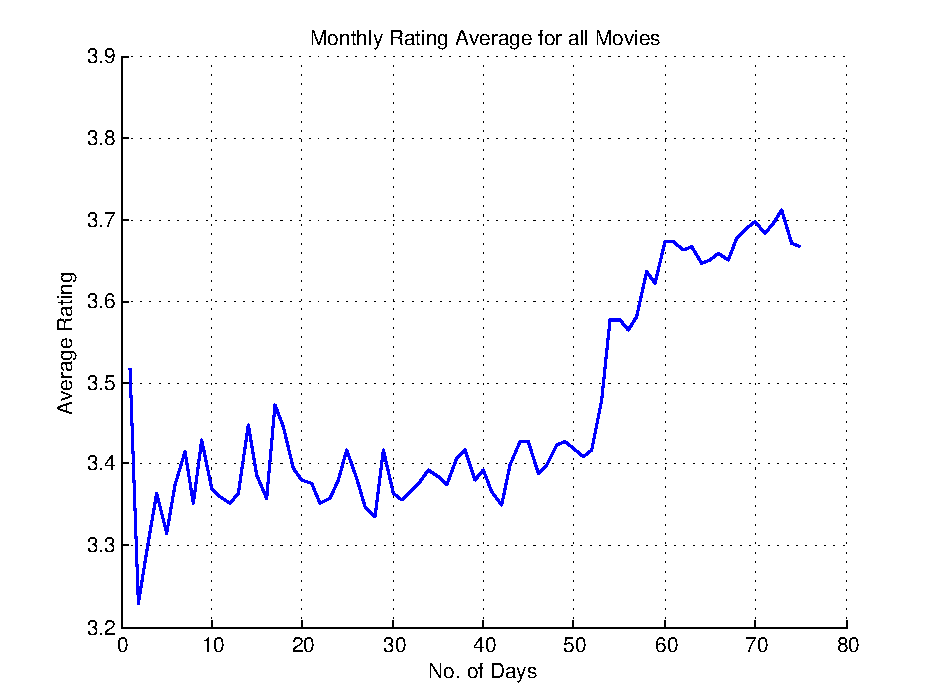
\includegraphics[width=0.45\textwidth]{./New/MonthlyAve_AllMovies.pdf}
\label{fig:MonthlyAllMov}
}
\subfigure[Weekly Average of all movies]{
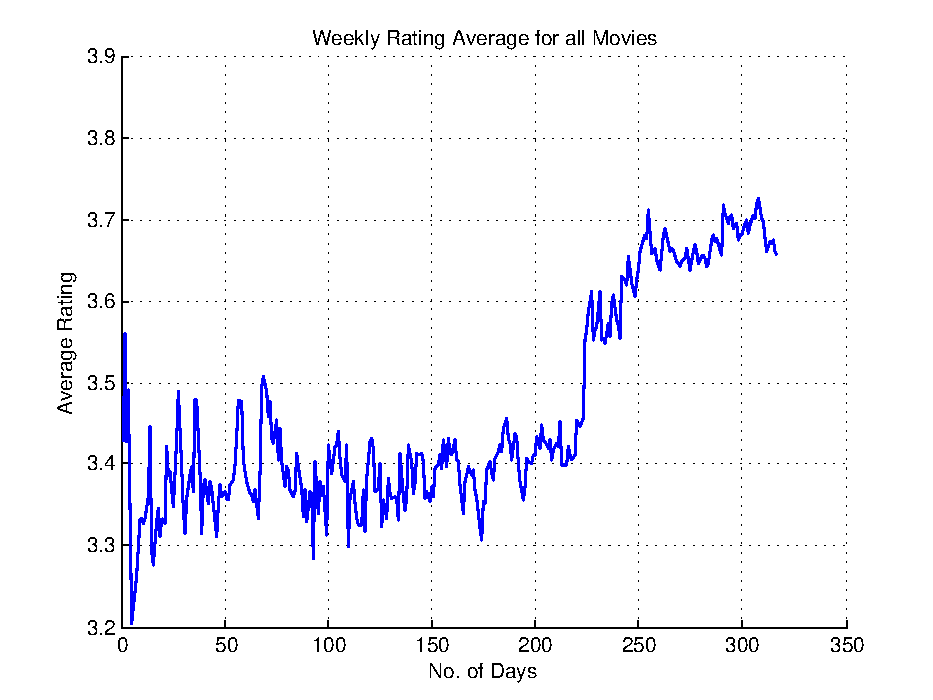
\includegraphics[width=0.45\textwidth]{./New/WeeklyAve_AllMovies.pdf}
\label{fig:WeeklyAllMov}
}\\

\subfigure[Monthly Average of movie 129]{
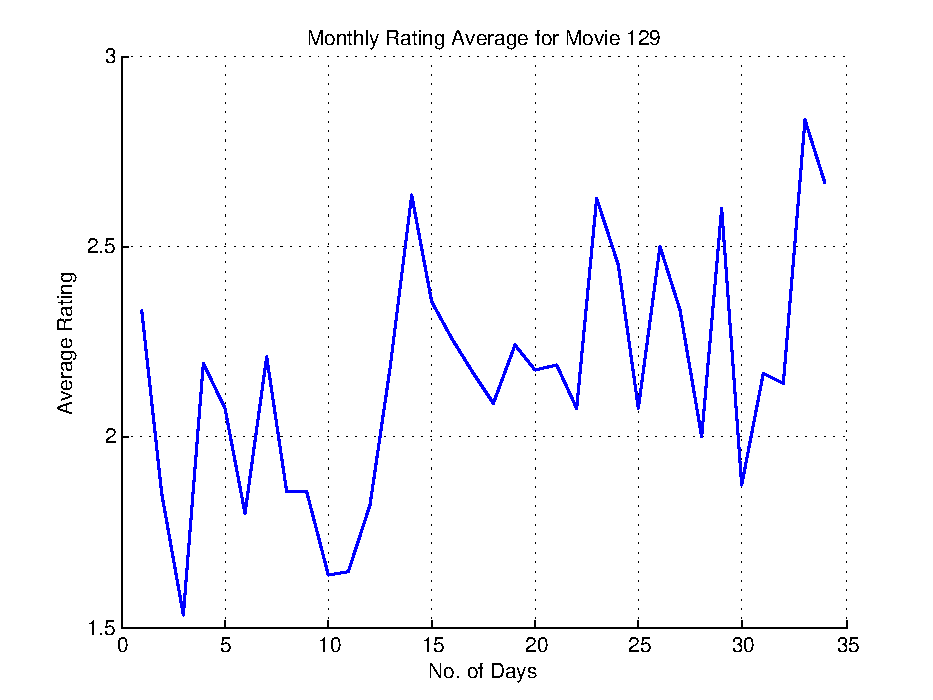
\includegraphics[width=0.45\textwidth]{./New/MonthlyAve_M129.pdf}
\label{fig:MonthlyM129}
}
\subfigure[Weekly Average of movie 129]{
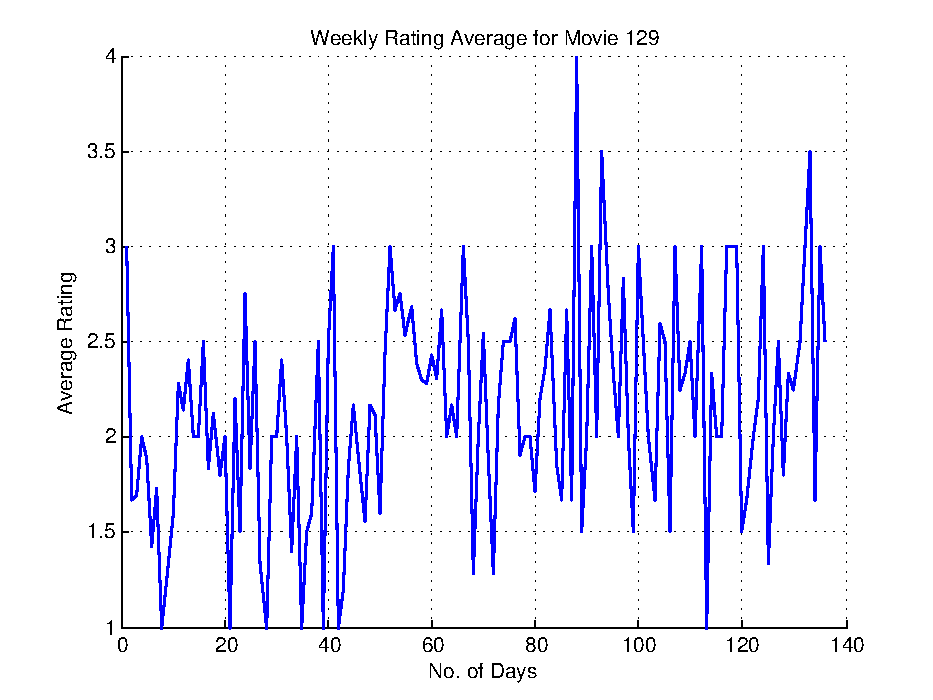
\includegraphics[width=0.45\textwidth]{./New/WeeklyAve_M129.pdf}
\label{fig:WeeklyM1476}
}\\

\subfigure[Monthly Average of movie 1476]{
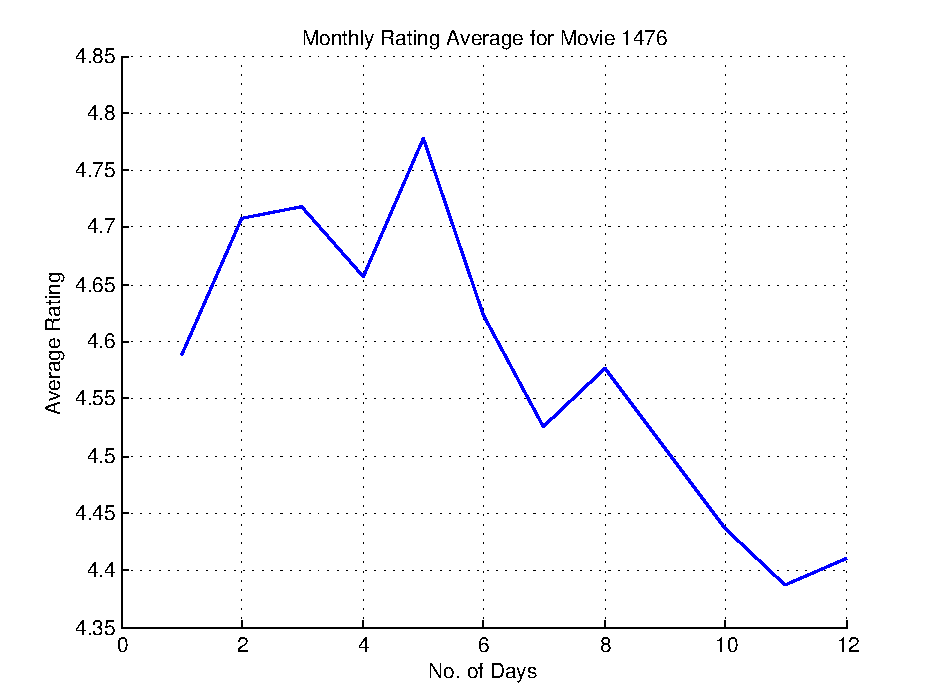
\includegraphics[width=0.45\textwidth]{./New/MonthlyAve_M1476.pdf}
\label{fig:MonthlyM129}
}
\subfigure[Weekly Average of movie 1476]{
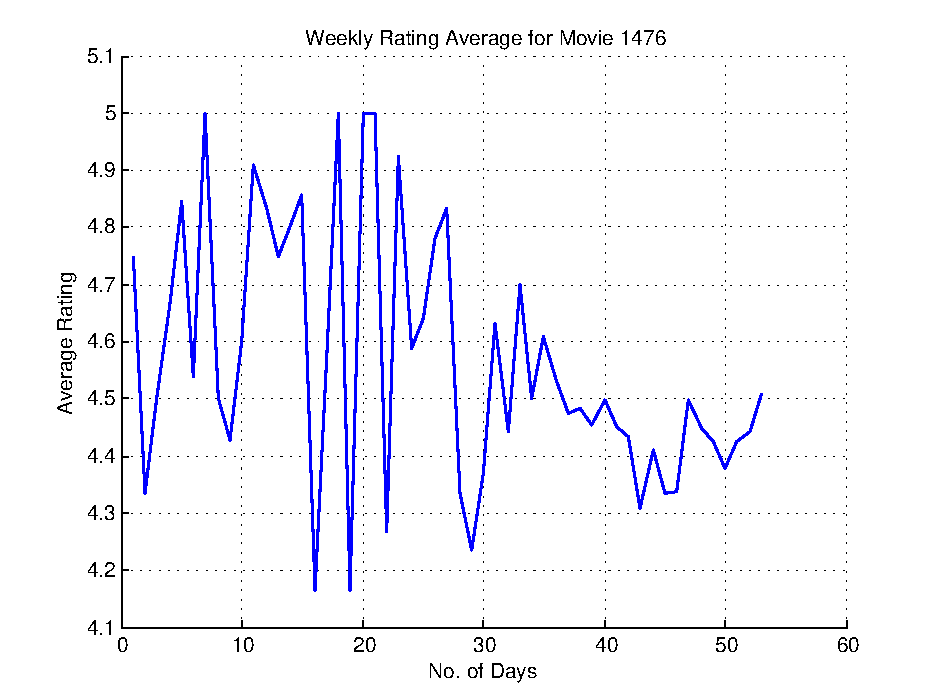
\includegraphics[width=0.45\textwidth]{./New/WeeklyAve_M1476.pdf}
\label{fig:WeeklyM1476}
}\\

\label{fig:MonthlyWeeklyAverages}
\caption{Monthly and Weekly Averages}
\end{figure}

We begun by experimenting for different time periods called \emph{bins} in order
to catch the movie-drifts.  The whole time period spans over 300 weeks, and
after several rounds of testing a 10 week period was chosen as the optimal bin
length. Hence a total of 30 bins suffice to span the entire data. With each bin
we associate it with a bias(transient part), which is simply the difference
between the overall movie mean and the mean of the movie for that bin period.
Interpolation is done for bins where there are no ratings. Each rating instance
of a movie in the training data is associated with a bin value between 1 and 30.
Hence the movie bias would have two components a stationary part, $b_{i}$ and a
transient part $b_{i,Bin(t)}$ \cite{Koren:2010:CFT:1721654.1721677}. \\

\begin{equation} 
 b_{i}(t)=b_{i}+b_{i,Bin(t)}
\end{equation}

We have in this thesis work considered only movie related temporal dynamics,
however we would comment on a possible approach to capture temporal dynamics
related to the more complicated user bias. In case users we need to parameterize
for both long term and short term changes. A simple linear function could be
used to capture the gradual user-bias drift. Each user will have an average
rating date, and for every rating instances of this user the deviation could be
a function of the difference of the dates. Regarding sudden drifts, we need to
capture the drift on daily basis. The minimum step length could be larger than a
day also. In the NETFLIX data the user on an average rates on 40 different days,
hence we need 40 different paramaters for every user on an average. These two
factors could model the temporal dynamics of the users.  


